\section{Perintah Dasar Bash}
\subsection{fungsi perintah pada Bash}

\begin{enumerate}
\item ls
	fungsi perintah \textbf{ls} pada bash ini yaitu untuk melihat isi dari suatu direktori. 
Contoh lihat pada gambar \ref{ls}
\begin{figure}[!htbp]
\centerline{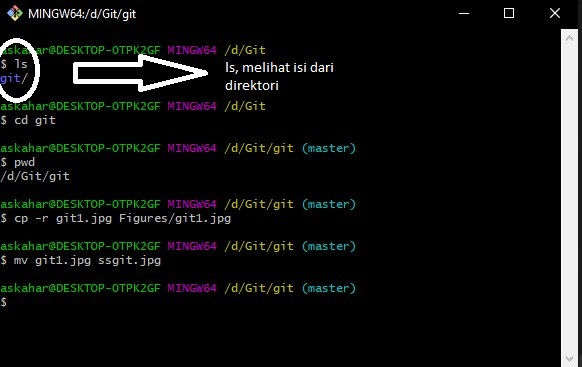
\includegraphics[width=.75\textwidth]{Figures/ls.jpg}}
\caption{Perintah dasar ls pada git bash}
\label{ls}
\end{figure}

\item cd 
	fungsi perintah \textbf{cd} \textit{(change directory)} pada bash ini yaitu untuk berpindah ke direktori yang dituju.
Contoh lihat pada gambar \ref{cd}
\begin{figure}[!htbp]
\centerline{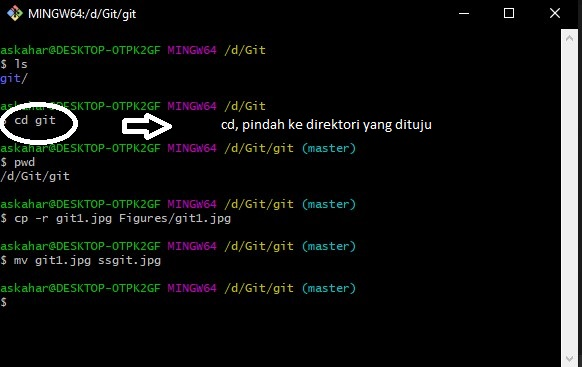
\includegraphics[width=.75\textwidth]{Figures/cd.jpg}}
\caption{Perintah dasar cd pada git bash}
\label{cd}
\end{figure}

\item pwd 
	fungsi perintah \textbf{pwd} pada bash ini yaitu untuk mengetahui path direktori yang sedang aktif.
Contoh lihat pada gambar \ref{pwd}
\begin{figure}[!htbp]
\centerline{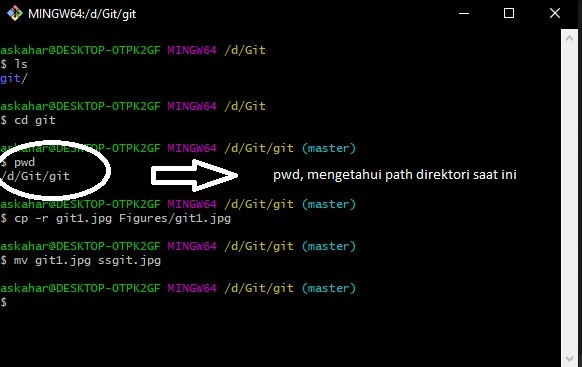
\includegraphics[width=.75\textwidth]{Figures/pwd.jpg}}
\caption{Perintah dasar pwd pada git bash}
\label{pwd}
\end{figure}

\item mv 
	fungsi perintah \textbf{mv} pada bash ini yaitu untuk mengubah nama file.
Contoh lihat pada gambar \ref{mv}
\begin{figure}[!htbp]
\centerline{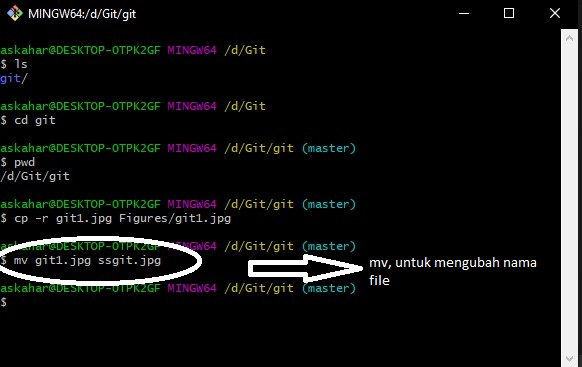
\includegraphics[width=.75\textwidth]{Figures/mv.jpg}}
\caption{Perintah dasar mv pada git bash}
\label{mv}
\end{figure}

\item cp
	fungsi perintah \textbf{cp} pada bash ini yaitu untuk men\textit{copy file}.
Contoh lihat pada gambar \ref{cp}
\begin{figure}[!htbp]
\centerline{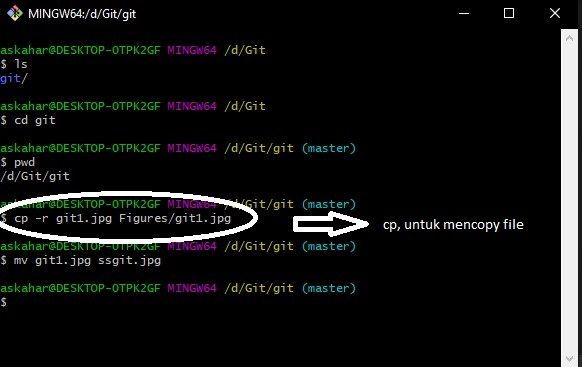
\includegraphics[width=.75\textwidth]{Figures/cp.jpg}}
\caption{Perintah dasar cp pada git bash}
\label{cp}
\end{figure}

\item :wq
	fungsi perintah \textbf{:wq} pada bash ini yaitu untuk keluar dari Vim editor ketika kita melakukan perubahan file menggunakan Vim editor.
Contoh ketika melakukan commit menggunakan VIM editor \ref{ss1}
\begin{figure}[!htbp]
\centerline{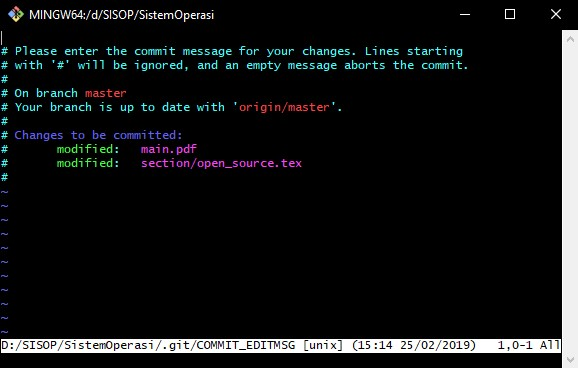
\includegraphics[width=.75\textwidth]{Figures/ss1.jpg}}
\caption{melakukan commit menggunakan VIM editor}
\label{ss1}
\end{figure}

selanjutnya setelah mengetikan commit maka akan masuk ke VIM editor tekan i pada keyboard sehingga kita dapat mengisi atau \textit{insert}, lalu isi apa yang kita commit \ref{ss2}
\begin{figure}[!htbp]
\centerline{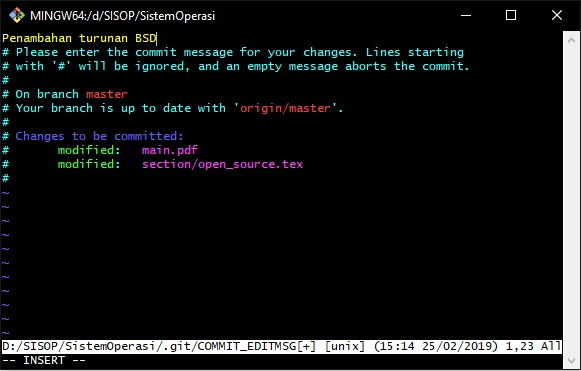
\includegraphics[width=.75\textwidth]{Figures/ss2.jpg}}
\caption{mengisi apa yang kita commit}
\label{ss2}
\end{figure}

jika, kita telah melakukan commit maka untuk keluar dari halaman VIM editor ini ketikan \textbf{:wq} untuk keluar dari halaman VIM editor \ref{ss3}
\begin{figure}[!htbp]
\centerline{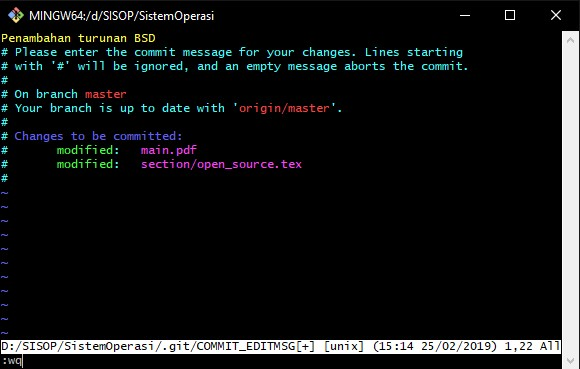
\includegraphics[width=.75\textwidth]{Figures/ss3.jpg}}
\caption{keluar dari halaman VIM editor}
\label{ss3}
\end{figure}
\end{enumerate}

 \subsection{penggunaan VI editor}
\begin{enumerate}
\item menambahkan file menggunakan VI editor di bash
\subitem ketikan vi namafile di bash untuk menambahkan file \ref{vi1}
\begin{figure}[!htbp]
\centerline{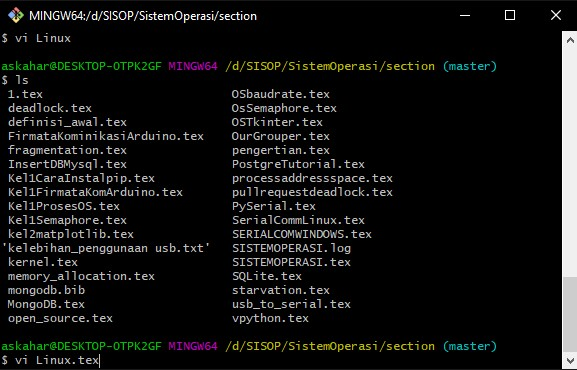
\includegraphics[width=.75\textwidth]{Figures/vi1.jpg}}
\caption{membuat file}
\label{vi1}
\end{figure}

\subitem lalu akan masuk ke halaman, tekan \textbf{i} untuk menambahkan isi file tersebut \ref{vi2}
\begin{figure}[!htbp]
\centerline{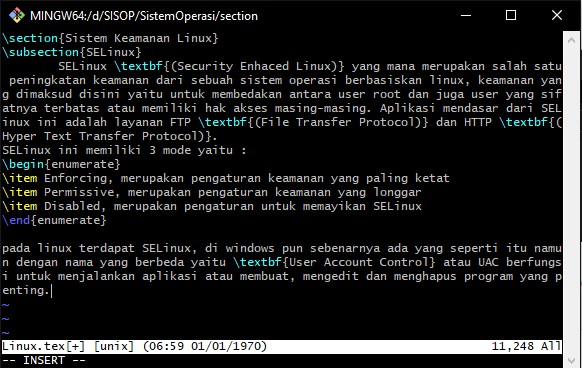
\includegraphics[width=.75\textwidth]{Figures/vi3.jpg}}
\caption{menambahkan data file}
\label{vi2}
\end{figure}

\subitem jika sudah mengisi data di dalam file untuk menyimpan file tersebut ketikan \textbf{esc} pada keyboard lalu \textbf{:w} untuk menyimpan file tanpa keluar dari halaman vi \ref{viw}
\begin{figure}[!htbp]
\centerline{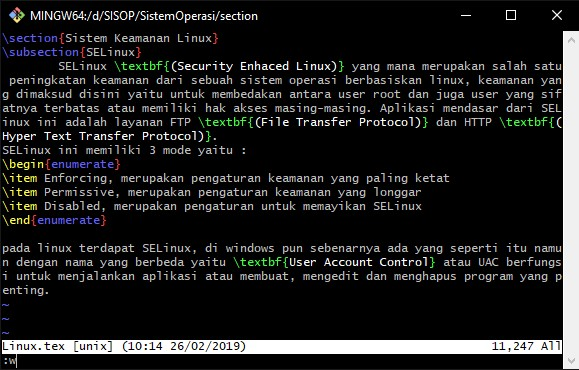
\includegraphics[width=.75\textwidth]{Figures/vi(w).jpg}}
\caption{menyimpan file}
\label{viw}
\end{figure}

\subitem untuk menyimpan file lalu keluar dari halaman vi maka ketikan \textbf{:wq} \ref{wq}
\begin{figure}[!htbp]
\centerline{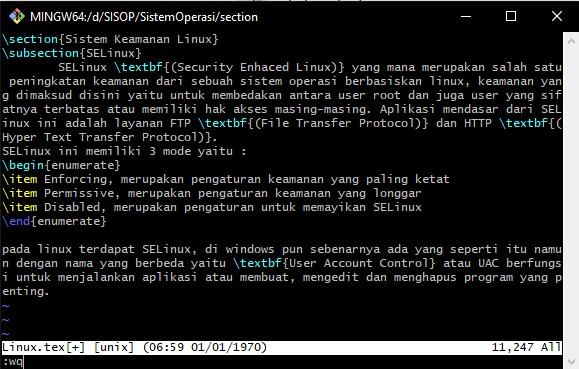
\includegraphics[width=.75\textwidth]{Figures/vi4.jpg}}
\caption{menyimpan file lalu keluar}
\label{wq}
\end{figure}

\subitem namun jika tidak ingin menyimpan atau mengubah file tersebut \textit{(discard all changes)} maka ketikan \textbf{:q!} \ref{q}
\begin{figure}[!htbp]
\centerline{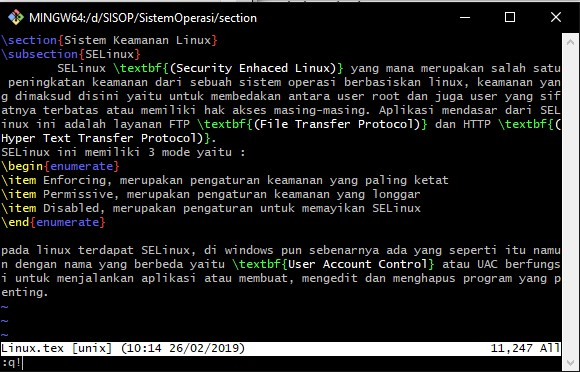
\includegraphics[width=.75\textwidth]{Figures/vi(q).jpg}}
\caption{keluar tanpa mengubah sesuatu pada file}
\label{q}
\end{figure}
\end{enumerate}

\begin{enumerate}
\item Fungsi dasar yang digunakan pada vi editor
\begin{table}[h]
		\begin{tabular}{|c|c|}
			\hline
			Perintah & Penjelasan\\
			\hline
			vi filename&Membuat file baru jika file belum dibuat, atau membuka file yang telah dibuat sebelumnya\\
			\hline
			vi -R filename&Membuka file yang sudah dibuat sebelumnya, namun hanya dapat dibaca tanpa bisa di edit\\
			\hline
			view filename&Sama seperti perintah sebelumnya hanya dapat membaca tanpa bisa melakukan edit\\
			\hline
		\end{tabular}
		\label{table:fungsi dasar}
	\end{table}

\item Menggerakan kursor di dalam file
\begin{table}[h]
		\begin{tabular}{|c|c|}
			\hline
			Perintah & Penjelasan\\
			\hline
			\textbf{k}&Menggerakan cursor ke atas satu baris\\
			\hline
			\textbf{j}&Menggerakan cursor ke bawah satu baris\\
			\hline
			\textbf{h}&Menggerakan cursor ke kiri satu karakter\\
			\hline
			\textbf{l}&Menggerakan cursor ke kanan satu karakter\\
			\hline
		\end{tabular}
		\label{table:menggerakan cursor}
	\end{table}
\end{enumerate}